\subsection{Downloading the game}
The game is published in the form of GitHub releases and can be downloaded from the address \url{https://github.com/Non-Euclidean-World/Hyper/releases}.
After every important improvement, a new release is shipped, so it's recommended to always download the latest version available.
A release, for example the one shown in \autoref{fig:release}, contains the following:
\begin{itemize}
    \item a ZIP archive with 64-bit Windows binaries (\texttt{win-x64}),
    \item a ZIP archive with 32-bit Windows binaries (\texttt{win-x86}),
    \item archives with the source code that the binaries were compiled from.
\end{itemize}

The application is published as \textit{self-contained} which means that it doesn't require any shared components to be installed on the target machine (even the .NET runtime).

\begin{figure}[H]
    \centering
    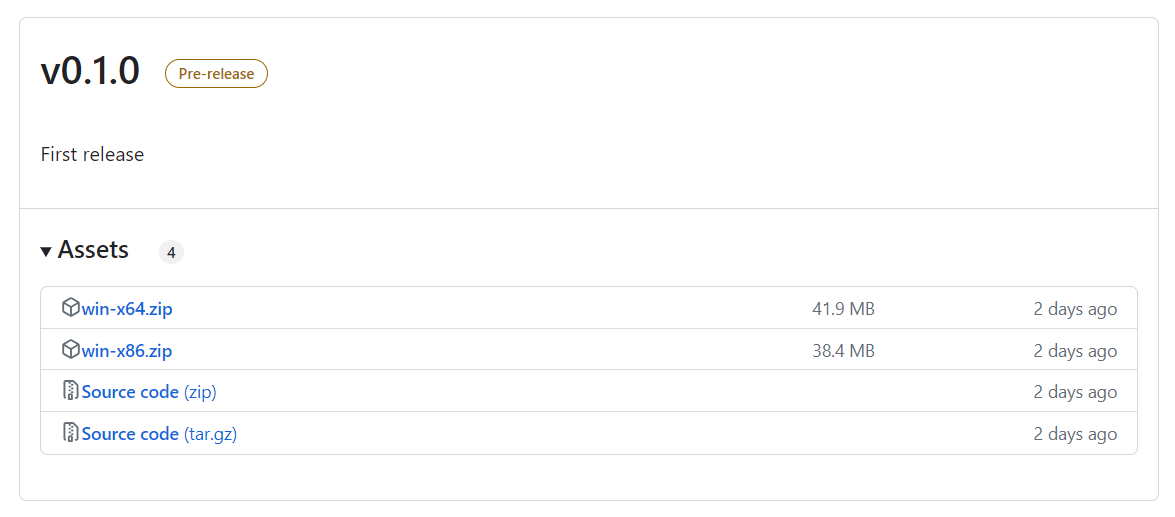
\includegraphics[width=0.8\textwidth]{sections/installation_instruction/resources/release-download.png}
    \caption{An example release}
    \label{fig:release}
\end{figure}

After unzipping the archive to a folder \texttt{<dest>}, the game, all of its required dependencies, etc. will be stored at \path{<dest>/Hyper-<release_version>} (the \textit{game folder}).
To launch the game, run the \texttt{Hyper.exe} executable from the aforementioned folder.